\section{Clases de com.example.prueba3.Clases}

Esta sección se dedica a la presentación de las Clases que constituyen el modelo de datos de la aplicación, ubicadas principalmente en el paquete `com.example.prueba3.Clases`. Como se indicó en la Figura \ref{fig:Diagrama_app_movil_detallado} (en la sección de Estructura Interna Detallada de la Aplicación Móvil), estas clases son fundamentales para la manipulación y el transporte de información dentro de la aplicación.

La mayoría de estas clases son Data Classes, un tipo de clase concisa en Kotlin diseñada específicamente para contener datos. Su función principal es servir como contenedores de información, estructurando los datos que se obtienen de los servicios remotos (a través de `RetroFit`), los que se manipulan dentro de la lógica de negocio, y los que finalmente se presentan en la interfaz de usuario a través de los `Views` (ViewModels). Estas clases aseguran la consistencia y la tipificación estricta de los datos a lo largo de todo el flujo de la aplicación.

A continuación, se mostrarán las imágenes de las Data Classes que conforman el paquete llamado `com.example.prueba3.Clases`. Cada imagen representará la estructura de una clase de datos, incluyendo sus propiedades (atributos) y tipos de datos, proporcionando una visión clara de cómo se modela la información esencial que fluye entre los componentes de la aplicación.

\newpage

\subsection{Diagrama de clases de com.example.prueba3.Clases parte 1}

La Figura \ref{fig:Clases1} muestra la primera parte del diagrama de clases de com.example.prueba3.Clases.

\begin{figure}[htbp!]
	\begin{center}
		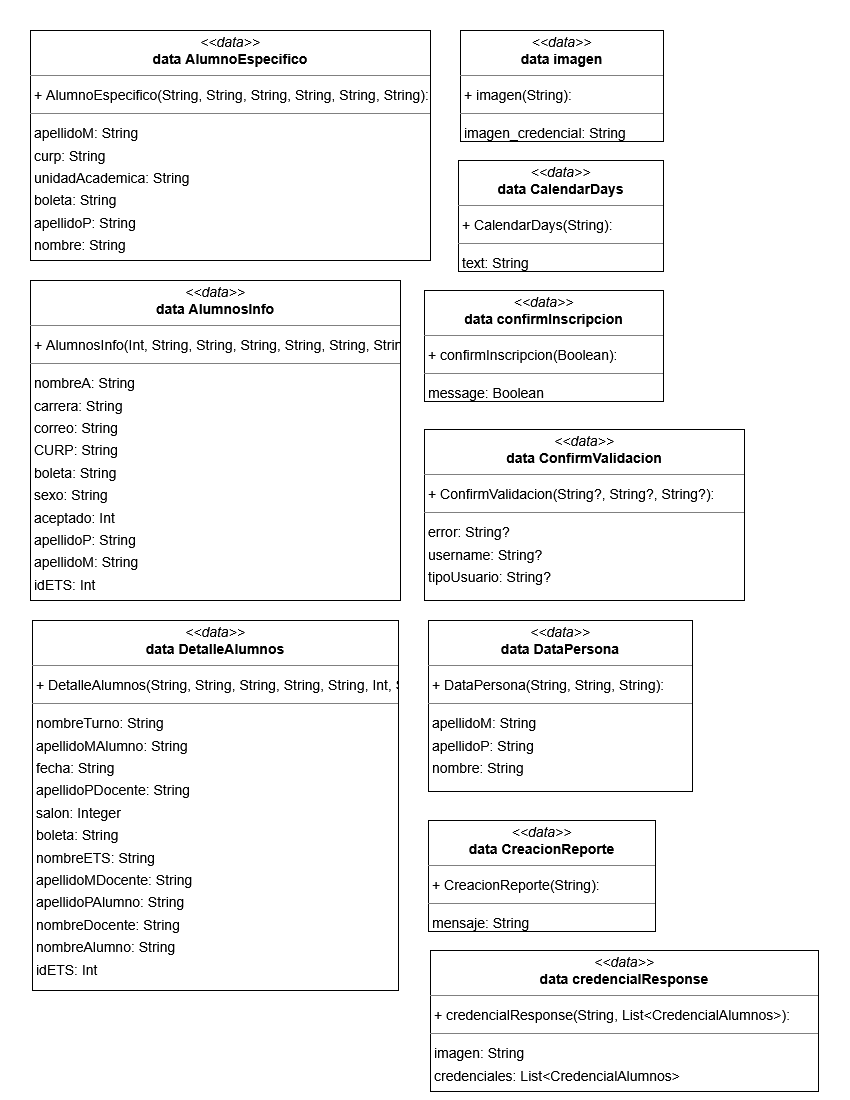
\includegraphics[width=0.75\textwidth]{DiagramasMoviles/DCM (2)}
		\caption{Diagrama de clases para com.example.prueba3.Clases parte 1.}
		\label{fig:Clases1}
	\end{center}
\end{figure}

\newpage

\subsection{Diagrama de clases de com.example.prueba3.Clases parte 2}

La Figura \ref{fig:Clases2} muestra la segunda parte del diagrama de clases de com.example.prueba3.Clases.

\begin{figure}[htbp!]
	\begin{center}
		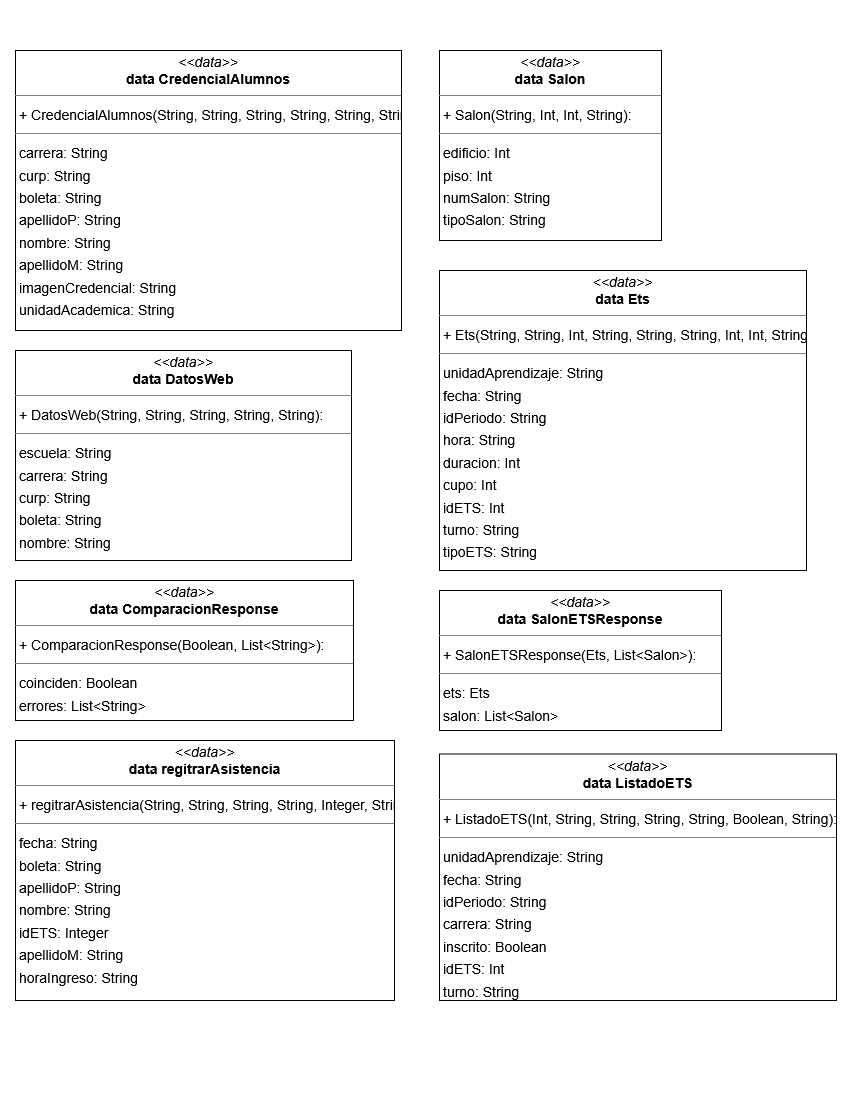
\includegraphics[width=0.75\textwidth]{DiagramasMoviles/DCM (3)}
		\caption{Diagrama de clases para com.example.prueba3.Clases parte 2.}
		\label{fig:Clases2}
	\end{center}
\end{figure}

\newpage

\subsection{Diagrama de clases de com.example.prueba3.Clases parte 3}

La Figura \ref{fig:Clases3} muestra la tercera parte del diagrama de clases de com.example.prueba3.Clases.

\begin{figure}[htbp!]
	\begin{center}
		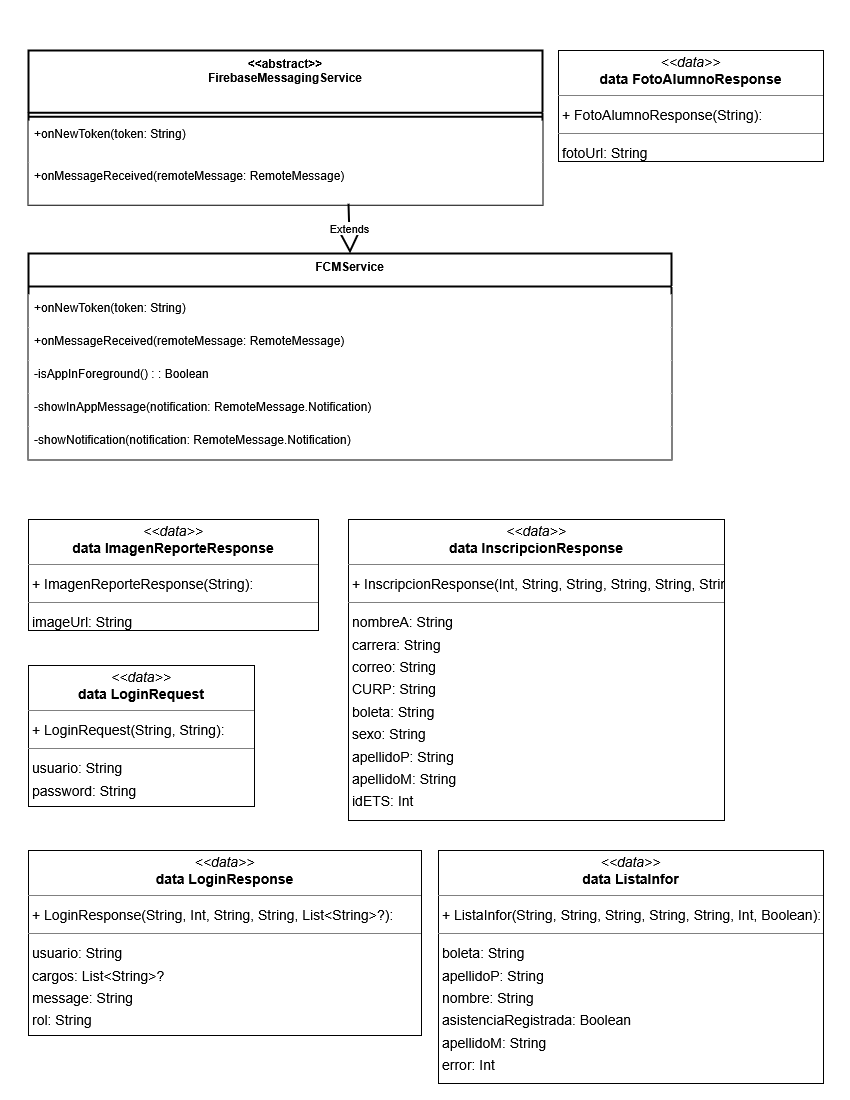
\includegraphics[width=0.75\textwidth]{DiagramasMoviles/DCM (4)}
		\caption{Diagrama de clases para com.example.prueba3.Clases parte 3.}
		\label{fig:Clases3}
	\end{center}
\end{figure}

\newpage

\subsection{Diagrama de clases de com.example.prueba3.Clases parte 4}

La Figura \ref{fig:Clases4} muestra la cuarta parte del diagrama de clases de com.example.prueba3.Clases.

\begin{figure}[htbp!]
	\begin{center}
		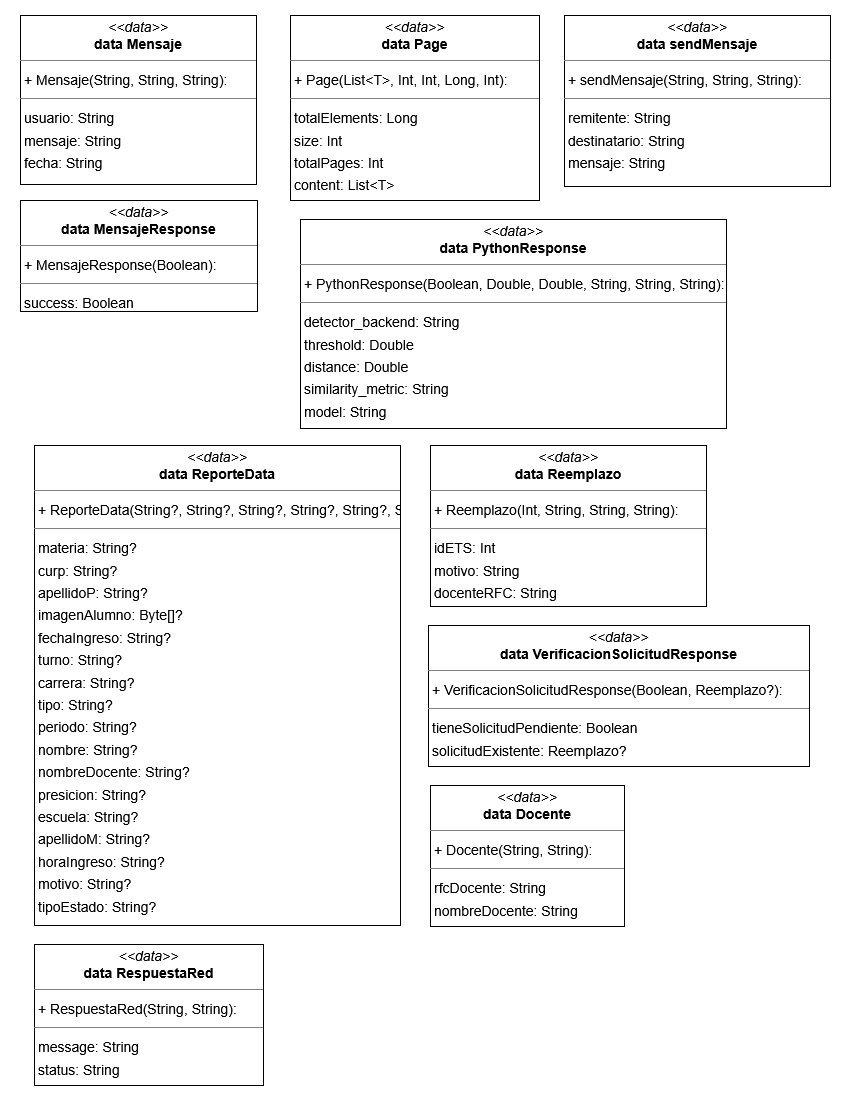
\includegraphics[width=0.75\textwidth]{DiagramasMoviles/DCM (5)}
		\caption{Diagrama de clases para com.example.prueba3.Clases parte 4.}
		\label{fig:Clases4}
	\end{center}
\end{figure}

\newpage

\subsection{Diagrama de clases de com.example.prueba3.Clases parte 5}

La Figura \ref{fig:Clases5} muestra la quinta parte del diagrama de clases de com.example.prueba3.Clases.

\begin{figure}[htbp!]
	\begin{center}
		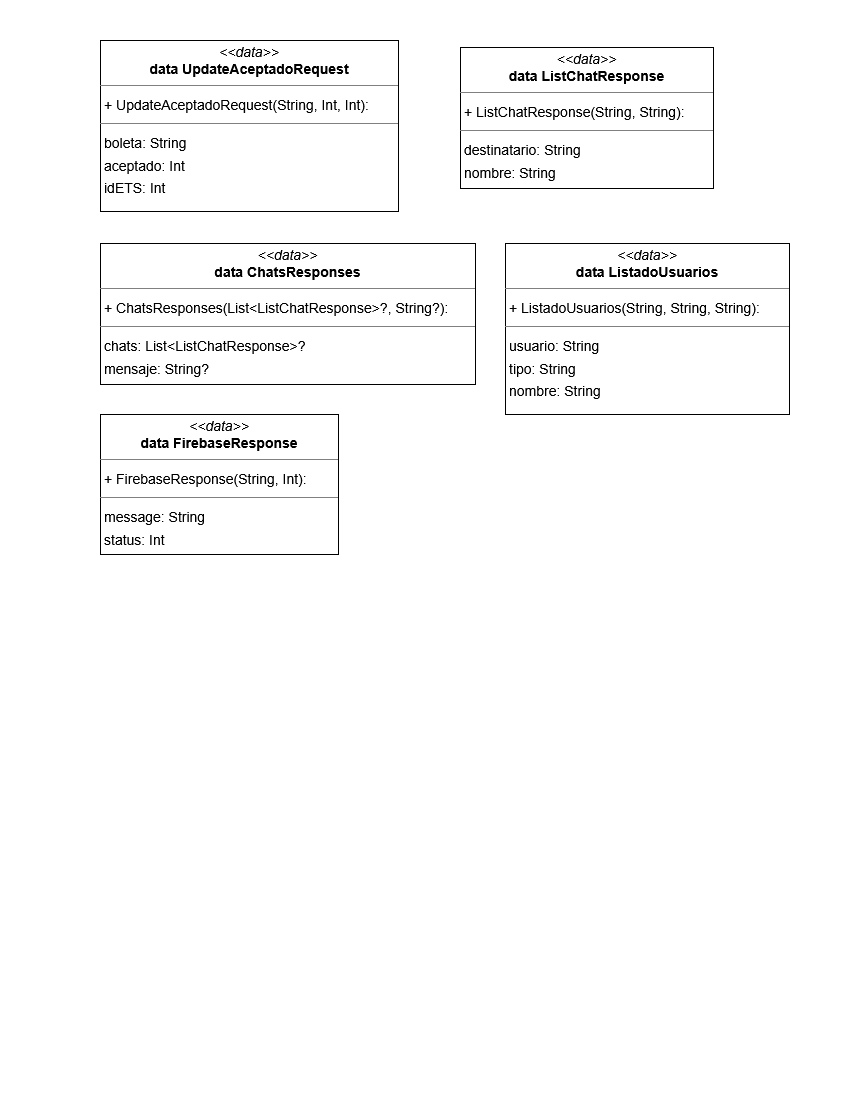
\includegraphics[width=0.75\textwidth]{DiagramasMoviles/DCM (6)}
		\caption{Diagrama de clases para com.example.prueba3.Clases parte 5.}
		\label{fig:Clases5}
	\end{center}
\end{figure}

\newpage